\documentclass[12pt, oneside]{report}

\usepackage[margin=2.5cm]{geometry}
\linespread{1.5}
\usepackage{hyperref}
\usepackage{mathptmx}
\usepackage{xcolor}
\usepackage{hyperref}
%\usepackage[style=authoryear, defernumbers=true, backend=biber,dashed=false, maxnames=999,maxcitenames=2,giveninits=true,urldate=long,uniquename=false,uniquelist=false]{biblatex}
\usepackage[
  sorting=none,
  backend=biber,
  style=ieee,
  citestyle=numeric-comp
]{biblatex}

\addbibresource{References.bib}
%\addbibresource{biblio.bib}

%% pretty captions
\usepackage{caption}
\usepackage{subcaption}
%%% allows you to create Rules, Definitions, Lemmas, Theorems etc.
\usepackage{amsthm}
\usepackage{amsmath}
\usepackage{amsfonts}
\usepackage[]{algorithm2e}

\newtheorem{theorem}{Theorem}
\newtheorem{definition}{Definition}
\newtheorem{lemma}{Lemma}
\newtheorem{Rule}{Rule}
\numberwithin{definition}{chapter}
\numberwithin{theorem}{chapter}  
\numberwithin{lemma}{chapter}  
\numberwithin{Rule}{chapter}  
\numberwithin{equation}{chapter} 
\newcommand\tab[1][1cm]{\hspace*{#1}}

 \usepackage[super]{nth} 
 
\usepackage{graphicx,graphics}
\usepackage{wrapfig}
\usepackage{placeins}
\usepackage{pdfpages}
\usepackage{attachfile2}

\usepackage[utf8]{inputenc}
\usepackage[T1]{fontenc}
\usepackage{csquotes}

\usepackage{fancyhdr}
%\pagestyle{fancy}
\renewcommand{\headrulewidth}{0.4pt}
%\renewcommand{\footrulewidth}{0.4pt}
\fancyhead{}
\fancyhead[L]{SHORTENED TITLE} %%% CHANGE AS APPROPRIATE (you may need to use a shortened form of the title)
\fancyhead[R]{Student ID: .......} %%% CHANGE AS APPROPRIATE
\fancyfoot{}
\fancyfoot[C]{\thepage}

\usepackage{titlesec}
\titlespacing{\chapter}{0pt}{*4}{*2.5}

\titleformat{\chapter}{\normalfont\huge\bf}{\thechapter}{20pt}{\huge\bf}
%% prevents Chapter 1 (then new line and Introduction) - turns into 1. Introduction


%% Call your references "References" rather than Bibliography, then also allow for a separate Bibliography if needed.

\DeclareSourcemap{
  \maps[datatype=bibtex]{
    \map{
      \perdatasource{references.bib}
      \step[fieldset=keywords, fieldvalue={, primary}, append]
    }
    \map{
      \perdatasource{biblio.bib}
      \step[fieldset=keywords, fieldvalue={, secondary}, append]
    }
  }
}
%%%%%%%%%%%%%%%%%%%%%%%%%%%%%%%%
%  Don't make any changes here
%  This defines formatting style
%%%%%%%%%%%%%%%%%%%%%%%%%%%%%%%%

\DeclareNameAlias{sortname}{last-first}
\DeclareFieldFormat{edition}{%
  \ifinteger{#1}
    {\ifnumequal{#1}{1}%
     {}%
     {\mkbibordedition{#1}~\bibstring{edition}}%
    }
    {#1\isdot}}

\DeclareFieldFormat[article,inbook,incollection]{title}{#1\isdot}
\DeclareFieldFormat[article,inbook,incollection]{citetitle}{#1\isdot}

\newrobustcmd{\MakeTitleCase}[1]{%
  \ifboolexpr{test {\ifentrytype{article}} or test {\ifentrytype{inbook}} or test {\ifentrytype{incollection}}}
    {#1}
    {\MakeSentenceCase{#1}}}

\DeclareFieldFormat{urldate}{\bibsentence\mkbibbrackets{\bibstring{urlseen}\space#1}}
\DeclareFieldFormat{url}{\bibstring{urlfrom}\addcolon\space\url{#1}}

\renewbibmacro*{journal}{%
  \iffieldundef{journaltitle}
    {}
    {\printtext[journaltitle]{%
       \printfield[titlecase]{journaltitle}%
       \setunit{\subtitlepunct}%
       \printfield[titlecase]{journalsubtitle}}
       \ifboolexpr{
         not test {\iffieldundef{url}}
         or
         not test {\iffieldundef{urldate}}
         or
         not test {\iffieldundef{doi}}
         or
         not test {\iffieldundef{eprint}}
       }
         {\nopunct\bibstring[\mkbibbrackets]{online}}%
         {}}}

\renewbibmacro*{journal+issuetitle}{%
  \usebibmacro{journal}%
  \setunit*{\addspace}%
  \iffieldundef{series}
    {}
    {\newunit
     \printfield{series}%
     \setunit{\addspace}}%
  \newunit
  \usebibmacro{volume+number+eid}%
  \setunit{\addspace}%
  \usebibmacro{issue+date}%
  \setunit{\addcolon\space}%
  \usebibmacro{issue}%
  \newunit}

\NewBibliographyString{online}
\DefineBibliographyStrings{english}{%
  urlseen    = {accessed},
  online     = {online},
}
%\addbibresource{example.bib}
\renewcommand*{\nameyeardelim}{\addcomma\addspace}
\renewbibmacro{in:}{%
  \ifentrytype{article}{}{\printtext{\bibstring{in}\intitlepunct}}} % removes "In" preceeding journal title
\setcounter{tocdepth}{1} % allow only sections (not subsections in table of contents)

\begin{document}
\begin{titlepage}
    \begin{center}
        \vspace*{1cm}
        {\huge
        Classifying and summarizing job offers in Switzerland with environmental activities using Natural Language Processing }
        \vspace{0.5cm}
        \\
        {\large By}
        \\
        \vspace{5mm}
        {\large Emily Sharata\\

        \vspace{1cm}
       
\includegraphics[width=0.7\textwidth]{logos/Logo_of_the_University_of_Geneva.jpeg}
       \\

        \vspace{5cm}      
        \begin{minipage}{10cm}
        \center A Master's dissertation submitted to the University of Geneva in accordance with the requirements of the degree of \textsc{Master of Business Analytics} in the School of Economics and Management.
        \end{minipage}\\
        \vspace{0.8cm}
        \today
        
}    \end{center}
  
 

\end{titlepage}
\newpage
\chapter*{Acknowledgements}
% Add here text if you would like to thank somebody, e.g., your family, friends, colleagues, supervisors, etc.

 I would like to thank my advisor Dr. Gilles Falquet for lending his knowledge and expertise to this research project. Thank you also to Marie-José Genolet Viaccoz and Sami Ghadfi for their help throughout the project. Finally, I would like to acknowledge my husband Kenneth for his unwavering support and encouragement.
 
 

\chapter*{Abstract}

This work investigates techniques for classifying 
job offers advertised in Switzerland according to whether or not they involve environmentally and non-environmentally related tasks. A method for extracting the advertised skills and activities of the job offers is also explored. This research builds upon work performed by the GE-EN-VIE network in semantic textual analysis.  A corpus of over 8000 job offers, provided by recruitment agency X28, are considered in the analysis. A binary classification model based on deep neural networks is built to categorize the job offers. Google's Universal Sentence Encoder is utilized to perform semantic textual similarity measures between the content of the job offers and a pre-compiled database of common environmentally related occupational skills and activities. Qualitative results of the categorization and textual similarity methods are discussed.  


    
 %% any other "Front matter" should go here before the table of contents - format in a style similar to the file Abstract.tex
\tableofcontents 
%\listoftables
% You don't actually have any tables so far...
\listoffigures
\addtocontents{toc}{~\hfill\textbf{Page}\par} % comment this line out if you want to remove "Page"
\label{sec:introduction}
\chapter{Introduction}
The focus of this research is to utilize artificial neural networks to classify a collection of job offers advertised in Switzerland as environmentally related or not, as well as to use Natural Language Processing (NLP) techniques to extract the work 
activities and skills from these said job offers. In particular, Google's pre-trained Universal Sentence Encoder (USE) is utilized to measure textual semantic similarity between the job offers and pre-defined databases of environmentally related skills and activities.

IE is a form of NLP in which specific types of information can be identified from text. 
Information such as user-defined keywords, relationships, dates, and events can be identified, classified, 
and extracted from documents, and then organized in a spreadsheet or database. IE is not to be confused with 
Information Retrieval (IR), in which a user generates a specific query and selects a relevant subset of documents 
from a larger collection~\cite{gaizauskas-wilks-1998-information}. Therefore, the focus of IE is on the gathering of specific information 
from texts or documents, while IR gathers the relevant documents from a larger corpus. In practice, these
two techniques are often used together in language processing. 

The history of modern IE can be traced back to the late 1980’s. The field developed quickly when the United States
Defense Advanced Research Projects Agency funded a large project aimed at extracting important information from naval 
messages in the US Navy~\cite{grishman_2019}. Experimental IE systems would be evaluated on their ability to accurately 
extract the messages of interest. During this time, the US government would host annual Message Understanding 
Conferences (MUCs) where various academic and industrial labs would compete to build the  best performing IE systems. 
Following the research surrounding the naval messages, these teams frequently worked with domains such as newswire articles. 
These historical conferences are of note because they represent the first widespread attempts at the development of large-scale, 
organized NLP systems. A result of these early years of research was the development of one of the first commercial IE 
systems called ATRANS, which could automatically process money transfer messages between banks~\cite{gaizauskas-wilks-1998-information}. 
A news fact extractor system called JASPER was developed for Reuters to help journalists quickly gather key facts to assist 
them in writing headlines more quickly. Larger, more complex IE systems developed in the 1990’s followed. These included systems 
such as vehicle fault report summarization, academic journal databases, employment opportunity databases, and police report 
summarization. While IE was indeed expanding into more diverse domains, the accuracy and recall of these systems were 
typically only around 50\%~\cite{gaizauskas-wilks-1998-information}.


In the 30 years since the inception of IE, the landscape of NLP has changed dramatically and the number of potential 
applications of IE has increased exponentially. As the Information Age has shifted into the Machine Learning Age, where 
crowdsourced or User Generated Data (UGD) produced by billions of users of smartphone, internet, and internet of things 
devices have rapidly improved Artificial Intelligence (AI) technology, we have begun to enter a time where computers can 
overtake human intelligence. AI technology surrounding natural text and language has advanced hugely in the past 10 years 
through supervised and unsupervised machine learning. It has given rise to disciplines and technologies such as sentiment 
analysis, where machines are able to recognize subtle nuances in text such as sarcasm and irony, virtual assistants, machine 
translation, document summarization, auto-correct, speech recognition, and text extraction. Everyday voice assistants including 
Amazon’s Alexa and Apple’s Siri are built on recent advances in NLP.  Within business settings, these tools can be used to help 
monitor and manage large amounts of unstructured text data such as email, social media conversations, customer service channels, 
market research queries, survey responses, and more. By automating many NLP tasks, companies can quickly and cost effectively 
gain better control over their data and drive better business decisions. 

% standard chapter format
\chapter{Presentation of research problem}
\label{chap:procedure}

Like many other countries globally, Switzerland is interested in the development and evolution of the sustainable and environmentally-focused sector of the job market. In particular, the Canton of Geneva has made an effort to fund research to understand the present situation of this sector.  The aim of the research detailed in this thesis is to utilize NLP techniques to analyze a corpus of environmentally related job offers published online in Switzerland between the years 2017-2021. This project is a collaboration among Geneva’s Département du territoire (DT), the Institute for Environmental Sciences at the University of Geneva, and l'Haute \'Ecole Du Paysage, D'Ing\'enierie et D'Architecture De Gen\`eve (HEPIA). Together, these three universities and public authorities form the GE-EN-VIE network that is intended to support knowledge and communication on the environment and improve the quality of life in the Canton of Geneva. The actions taken by the network are designed to support the ``climate, energy, and biodiversity'' pillar of the Federal Office for Spatial Development’s 2030 Strategy for Sustainable Development. One of these concerns revolves around the dynamics and the evolution of the environmentally-focused labor market in Switzerland. The GE-EN-VIE network has found it necessary to gain a deeper understanding of the sector in order to better prepare job seekers for the market, to measure the presence of environmental job functions in Switzerland, and to assess the future needs to continue to support companies on their journeys to becoming more ecologically sustainable.

	Therefore, the aim  of this research is to analyze the specific skills and activities that are present in the corpus of job offers, building upon work that has been headed by Marie-José Genolet Viaccoz, a leader within the Institute for Environmental Sciences. Over 8000 job offers were obtained by the company X28, who provide detailed labor market data that were selected for their environmental character. A preliminary semantic analysis was performed by the GE-EN-VIE researchers to gain an understanding of the most common skills and activities in a subset of the job offers. These skills and activities were then compared and classified according to those organized by O*Net, a free online database that contains hundreds of occupational definitions. In this way, the researchers were able to link pre-defined skills and activities to the job offers, and measure their evolution over time. This research will build upon the work already completed by the GE-EN-VIE team with the objective of extracting the most frequent activities contained in the job offers, and matching them to the environmentally-related skills and activities contained in the O*Net-extracted data set, which provides a standard for each skill and activity.

\section{Software and analysis tools}
\label{sec:software}
The primary focus of this research work is building a software infrastructure to classify and categorize environmentally-focused jobs. The programming language Python is used to develop software to perform all steps of processing and analyzing the text data and interpreting the results. The software library developed for this task can be found in Ref.~\cite{emilysharata}. Common functions for processing and cleaning the data or stored in the Methods directory, and individual Jupyter notebooks are used to drive the individual tasks of the project: categorizing job offers as environmentally-focused or not, associating offers to specific skills, and associated job offers to tasks.

The basic tasks of the software are:

\begin{itemize}
\item Read the available job offers data from a JSON file format.

\item Clean the job description text of non-textual characters and symbols.

\item Convert the text into numeric data necessary for the machine learning tasks.

\item Perform analysis, associating the numeric encoding of the job offers to activities and skills, and using machine-learning algorithms to categorize the jobs.

\item Interpret the results, assessing performance numerically and/or qualitatively.
\end{itemize}

The following Python software libraries are utilized to aid these tasks.

\begin{itemize}
    \item \textbf{pandas}~\cite{reback2020pandas,mckinney-proc-scipy-2010} -- A multifunctional library that assists with loading and reading a variety of input file formats, including JSON and CSV files, building dataframes, and handling missing data. This library is used extensively to provide a convenient and flexible interface to the data for processing.

    \item \textbf{googletrans} -- An implementation of the Google Translate web API, this package queries the Google Translate webpage to build translations. It is used to convert the job offers in other languages, especially German, French, or Italian, into English.

    \item \textbf{BeautifulSoup}~\cite{richardson2007beautiful} -- A Python library for pulling data out of HTML and XML files. It is used to clean the job offers of HTML tags and non-alphanumeric characters, as the text has generally been scraped from webpages and may contain superfluous characters.

    \item \textbf{EasyNMT}~\cite{TiedemannThottingal:EAMT2020} -- EasyNMT stands for easy neural machine translation. This package provides machine translation and detection for over 150 languages. This package is slower than googletrans, but it is more robust, so it is used to translate job offers into English when the googletrans package fails

    \item \textbf{NumPy}~\cite{harris2020array} - NumPy stands for numerical Python. This package was designed to facilitate the use of arrays in Python. It is used to process arrays and for many statistical operations.
    
    \item \textbf{TensorFlow}~\cite{tensorflow2015-whitepaper} - Created by Google, TensorFlow is a package created for fast and efficient numerical computing. It is used in tandem with the Keras package to build machine learning models.

    \item \textbf{Keras}~\cite{chollet2015keras} - A library that provides an interface for building artificial neural neural networks, which will be discussed in more detail later in this thesis. The library has the capability of deploying many common components of neural networks including layer configurations, activation functions, and optimizers. It is used to build the neural network used for environmental job categorization described in Section~\ref{sec:classification}.
    
    \item \textbf{Universal Sentence Encoder}~\cite{DBLP:journals/corr/abs-1803-11175} - A pre-trained model that encodes text into high dimensional numerical vectors that can be used for textual semantic similarity, clustering, information retrieval, and other natural language tasks.  
    
    \item \textbf{TensorFlow Hub}~\cite{tensorflow2015-whitepaper} - A repository that houses a number of pre-trained models, including the Universal Sentence Encoder, ready for practical application. 
    
    \item \textbf{SciPy}~\cite{2020SciPy-NMeth} - A Python library that consists of a large suite of tools for statistical analysis and machine learning. It is used for statistical operations, especially for the cosine distance calculation used for the sentence similarity task of Section~\ref{sec:activites}.  
    
    \item \textbf{matplotlib}~\cite{4160265} -- A graphics package used to visualize and explore the data set.
    
    \item \textbf{Jupyter notebook}~\cite{Kluyver2016jupyter} -- A visual interface to Python, used to provide a convenient and visual work environment analogous to RStudio.
    
\end{itemize}
Like many other tasks in NLP, this problem is challenging because there exists no training data. This makes it difficult to build certain deep learning models. Annotating data in text form can be costly, difficult, and time consuming, making the evaluation of many NLP tasks strenuous. Very few large scale training sets are available for research or industrial NLP tasks~\cite{DBLP:journals/corr/abs-1803-11175}. Even for humans, labelling, extracting information, and categorizing text can be a challenge. For a computer, processing human languages can be difficult for a number of reasons. Real-world text data can be incomplete, inconsistent, illogical, contain various character encodings, or have special characters. Human language is complex and can be filled with nuance. Word order and context can completely change the intrinsic meaning of a sentence. In natural language, words can have different meanings based on syntax or semantics. For example, the word book can be either a noun or a verb based on context, such as ``I read a book,'' or ``I booked a vacation.'' In even more challenging scenarios, sentences can have more than one reasonable interpretation. ``I saw the dog on the beach with my binoculars'' could have an ambiguous meaning. It could mean to infer that the subject saw the dog through the subject’s binoculars, or alternatively that the dog on the beach was in possession of the subject’s binoculars. In order to understand the intended meaning, it would be necessary to have the full context of the sentence within a paragraph or larger corpus. 

In addition to the challenge posed by the lack of annotated training data in this research problem, there exists many other complications with the job offer corpus compiled by X28. The largest problem is that a large number of job offers are not actually environmentally related. Although they are meant to be selected for their environmental nature, the corpus includes non-green job offers for positions such as quality manager, watch makers, building managers, and pharmaceutical technicians. Furthermore, an-insignificant number of offers contains little to no text, or are incomplete or incomprehensible. The text throughout the corpus also are filled with special characters and HTML text formatting elements, making it difficult to read. Finally, the corpus contains text written in English, French, Italian, and German. 
Given the objectives of the research and the quality of the data provided, the research tasks are split into two tasks. The first task specified is to design a classifier that can split the job offers into ``environmentally related” and ``non environmentally related” categories, and the second task specified is to extract the specified activities and skills in each job offer, and match them to the standard activity and skill database compiled from O*Net. A methodology for each task is needed to be designed to produce results with little to no training data, as none are available at the time of this research.

To address the first challenge of building an “environmentally related” and “non environmentally related” classifier, an artificial neural network is built using the Python package Keras. The benefits of using neural networks or other deep learning models for NLP tasks is that learning can be done unsupervised, and that these models can also handle the recursivity of natural language, which are composed of complex word and sentence structures~\cite{10.5555/3208611}. With regards to the second task, extracting the specified activities from each job offer, an approach utilizing semantic sentence similarity is chosen. Within NLP, semantic similarity refers to a task that outputs a score of the relationship between two different texts. The most common way to accomplish this is to use a model that encodes the individual sentences in the text to obtain their embeddings, and then computes the numerical distance between the embeddings, most commonly with a cosine distance. This type of approach is again chosen as a practical option because it can be used without any training data.

Prior to implementing either of these strategies, the first steps taken are to clean the job offers corpus and to remove the HTML tags and special characters. A function is written to only allow UTF-8 encoded alphanumeric characters. Next, the text is split on periods into individual sentences. This process in NLP is called tokenization. Tokenization is a way of splitting larger pieces of text into smaller units. This is done so that textual analysis can be done on a smaller level, allowing for faster processing and more precise identification and location of certain information. Following tokenization, the Python package EasyNMT was used to translate the corpus entirely into English for uniformity and for the ability to manually inspect the results of the analyses. 

\label{sec:dataset}
\section{Data set exploration}

The job offers corpus contains 8565 job offers written in French, English, German, and Italian and contains positions from a wide range of Swiss cantons. Below is a description of each variable in the job offers data set:

\textbf{JOB ID}: A unique numerical identifier assigned to each job offer in the corpus.

\textbf{ISCO}: An identifier that relates the job posting to the Swiss Standard 	
Classification of Occupations (CH-ISCO-19). This fact sheet is published by the Federal
Statistical Office and is used for several federal labour market surveys. 

\textbf{SKILLS}: A list of text keywords describing the skills, sectors, or industries related to each job offer.

\textbf{CANTON}:The canton the job offer was originally advertised in. 

\textbf{WORK EXPERIENCE}: A list of keywords describing job titles related to each job offer.

\textbf{EDUCATIONAL LEVEL}: The educational experience desired by each job offer.

\textbf{DATE}: The date the job offer was published. 

\textbf{COMPANY}: The name of the company advertising the job offer. 

\textbf{JOB TITLE}: The official job title of the job offer. 

\textbf{JOBS}: A list of keywords related to the official job title.

\textbf{CONTENT}: The raw text of the job offer, written in French, English, German, Italian, or some combination. 

Data sets of environmentally-related skills and activities were also compiled by the GE-EN-VIE researchers in order to create reference documents to match the contents of the job offers to. Below of is a description of the activities data set:

\textbf{ACTIVITY ID}: A unique numerical ID assigned to each environmentally related activity.

\textbf{O*Net - All the jobs}: A short list of broad keywords that describe the category of skills the detailed activities fall under. 

\textbf{O*Net - Green jobs}: A unique numerical ID assigned to each activity description.

\textbf{O*Net - Details of the activities for green jobs }: A sentence describing each occupational activity in detail, as listed in the O*Net database. 

\textbf{Terms (verbs) found in the 120 "environment" job offers}: A list of individual verbs related to the sentences of detailed activities.

\textbf{Terms (adjectives) found in the 120 "environment" job offers}: A list of individual adjectives related to the sentences of detailed activities. 

The description of the data set of the environmentally-related skills is as follows: 

\textbf{SKILL ID}: A unique numerical ID assigned to each environmentally related skill.

\textbf{SKILL}:  A sentence describing each occupational skill in detail, as listed in the O*Net database. 

To assist with the automatic classification of environmentally related and non-environmentally related jobs, a total of 536 jobs were manually labeled as such by Marie-José Genolet Viaccoz. In addition, a total of 1000 jobs from the job offers corpus were analyzed in an exploratory analysis to gain a better understanding of the data set. 

The distribution of jobs by location, shown per canton in Switzerland, is shown in Fig.~\ref{fig:cantons}. The majority of the jobs postings are for positions in Bern and Vaud, followed by Geneva. Of all the cantons, Geneva has the highest ratio of environmental jobs to non-environmental jobs. 

\begin{figure}[htbp]
  \centering
    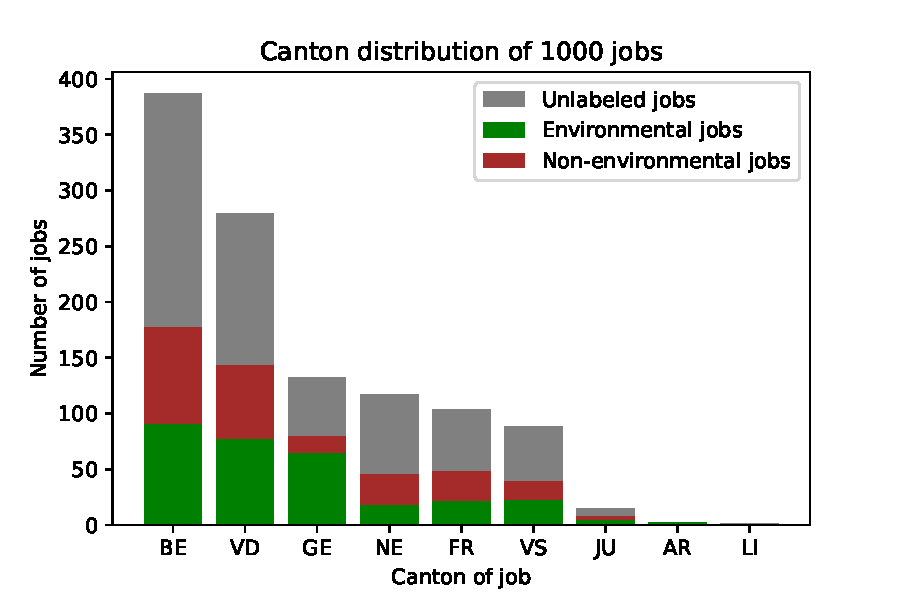
\includegraphics[width=0.49\textwidth]{figures/CantonDist.pdf}
    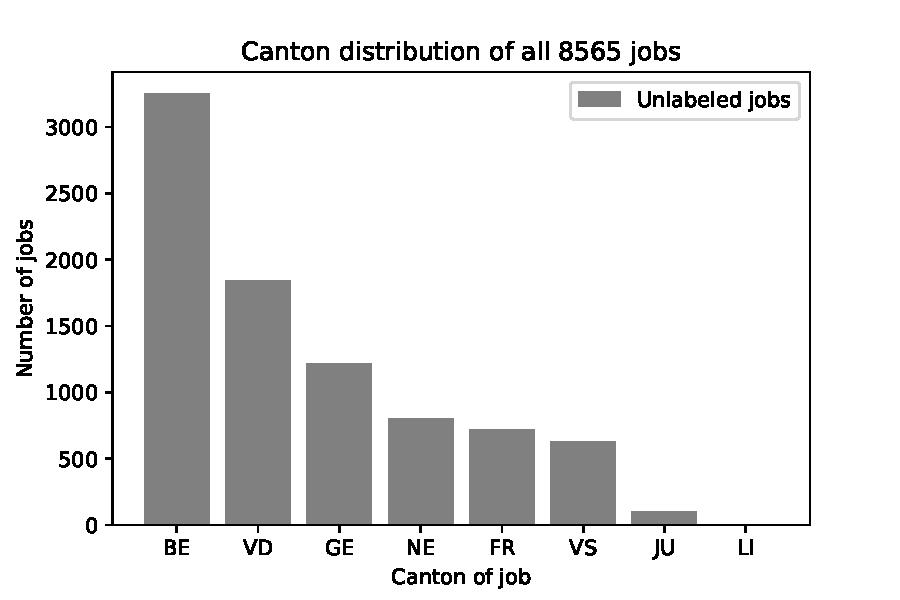
\includegraphics[width=0.49\textwidth]{figures/CantonDistAll.pdf}
    \caption[The distribution of job locations by canton in Switzerland]{
    	The distribution of job locations by canton in Switzerland.
        The left plot shows a subset of 1000 jobs, of which nearly half are labeled to indicate if they are environmental. The right plot shows the distribution for all 8565 jobs.
        Jobs categorized as environmental are shown in green, and those that are not environmental are shown in red.
        The portion of the data set that has not been categorized is shown in grey. The right plot shows the distribution
        of all 8565 jobs in the data set.
    }
\label{fig:cantons}
\end{figure}

Most of the jobs in the data set were sourced from small or midsize companies. The proportion of environmentally related jobs to non-environmentally related jobs is relatively consistent across company size, as seen in Fig.~\ref{fig:companysize}.

\begin{figure}[htbp]
  \centering
    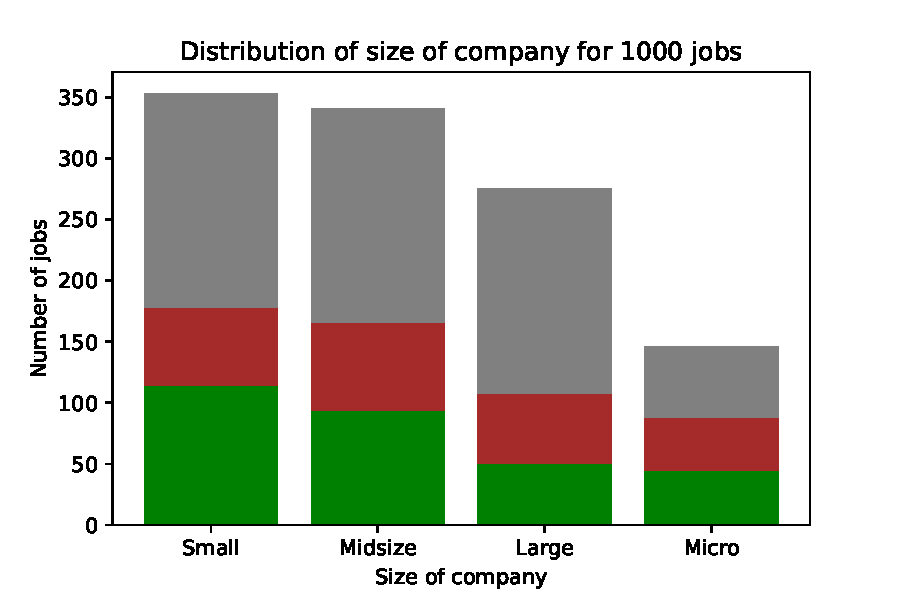
\includegraphics[width=0.49\textwidth]{figures/CompanySize.pdf}
    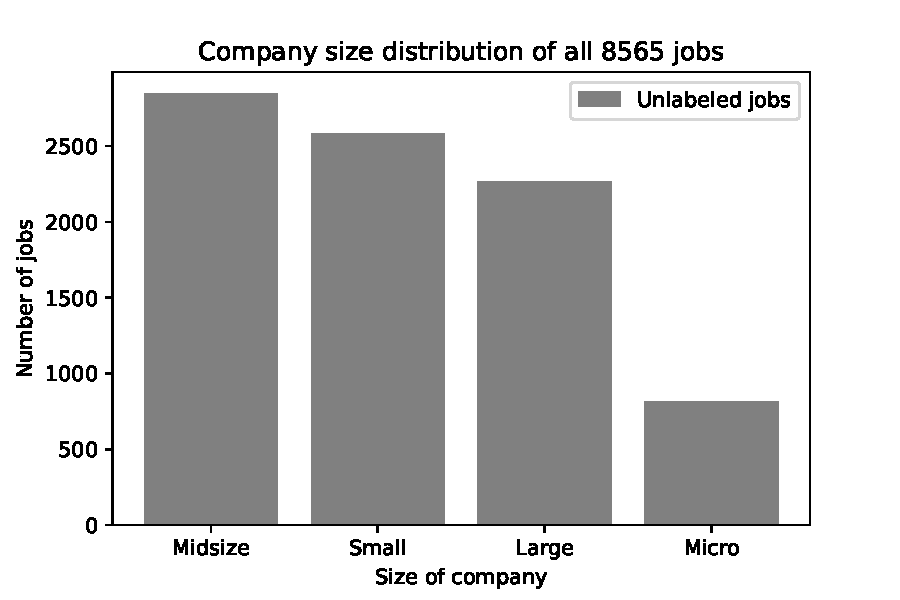
\includegraphics[width=0.49\textwidth]{figures/CompanySizeAll.pdf}

    \caption[The distribution of company size in the jobs data set]{
    	The distribution of company size.
    	The left plot shows a subset of 1000 jobs, of which nearly half are labeled to indicate if they are environmental. The right plot shows the distribution for all 8565 jobs.
        Jobs categorized as environmental are shown in green, and those that are not environmental are shown in red.
        The portion of the data set that has not been categorized is shown in grey. The right plot shows the distribution
        of all 8565 jobs in the data set.
    }
\label{fig:companysize}
\end{figure}



With regards to the number of sentences in each job description, a greater number of non-environmentally related jobs had descriptions with fewer sentences, as seen in Fig.~\ref{fig:sentencelength}. Many of these job descriptions do not contain enough information about the job or company to be classified as environmentally related.


\begin{figure}[htbp]
  \centering
    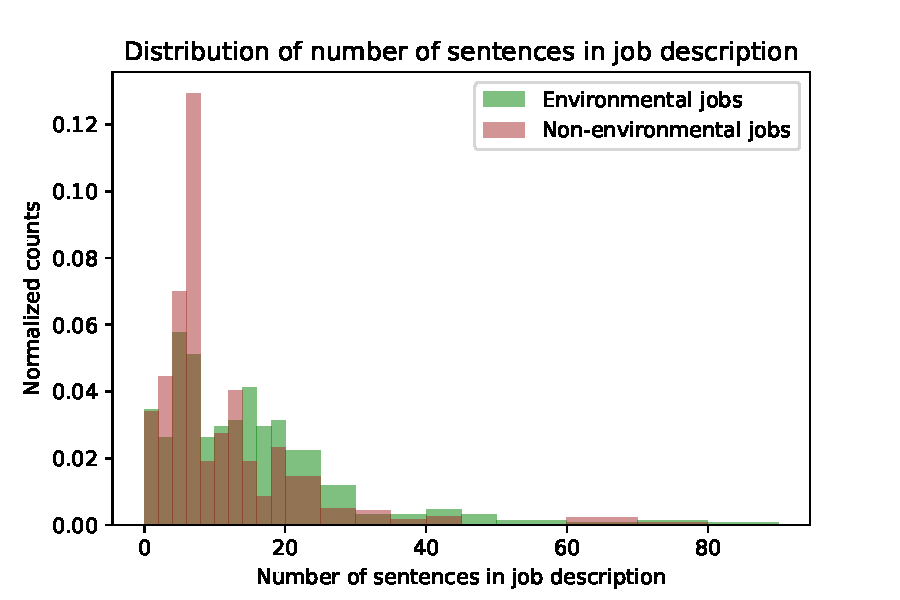
\includegraphics[width=0.49\textwidth]{figures/SentenceLength.pdf}
    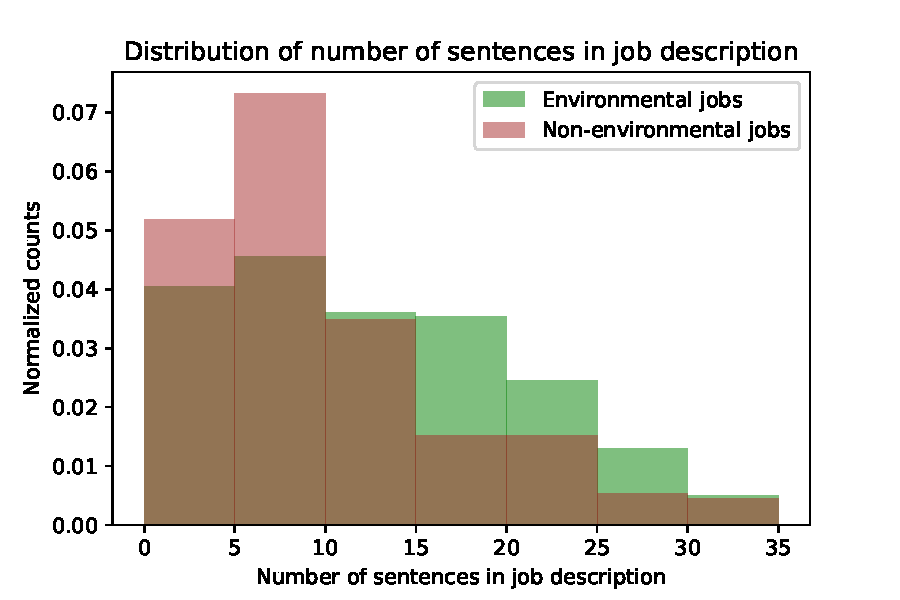
\includegraphics[width=0.49\textwidth]{figures/SentenceLengthZoomed.pdf}

    \caption[The distribution of the number of sentences in each job description]{
    	The distribution of the number of sentences in each job description.
    	The left plot shows the densities of the 536 labeled jobs. The right plot shows the same subset of jobs, but on a range from 0-35 sentences. 
        Jobs categorized as environmental are shown in green, and those that are not environmental are shown in red.
    }
\label{fig:sentencelength}
\end{figure}


The distribution of the number of sentences in the entire data set is similar to that of the subset of 536 labeled job offers, as seen in Fig.~\ref{fig:sentencelengthall}. The vast majority of the job offers contain fewer than 20 sentences. 

\begin{figure}[htbp]
  \centering
    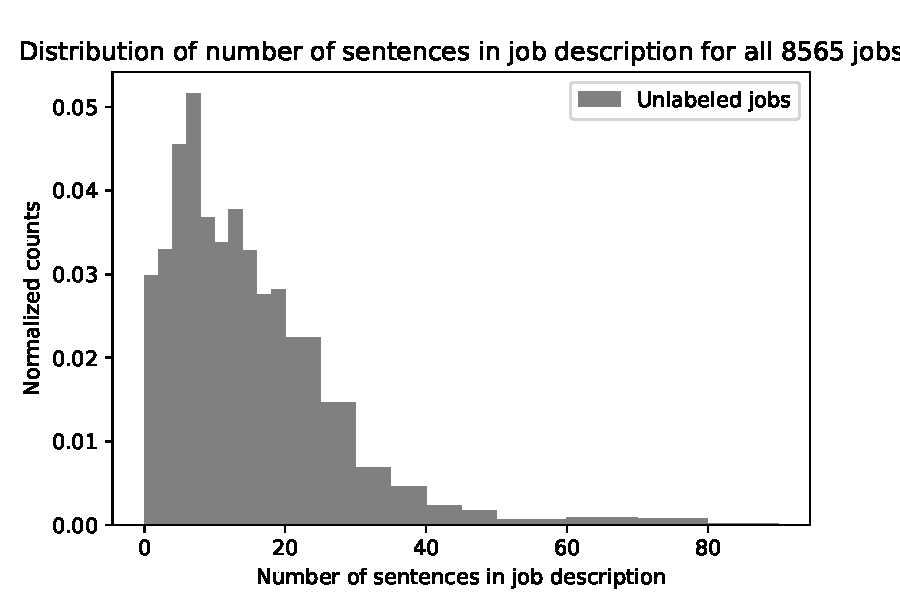
\includegraphics[width=0.49\textwidth]{figures/SentenceLengthAll.pdf}
    \caption{
    	The distribution of the number of sentences in all 8565 job descriptions.
    }
\label{fig:sentencelengthall}
\end{figure}


A large number of job descriptions in the data set have fewer than 200 characters as seen in Fig.~\ref{fig:charlength}. Likewise, as with the number of sentences, job descriptions with small amounts of text are more frequently classified as as non-environmentally related.

\begin{figure}[htbp]
  \centering
    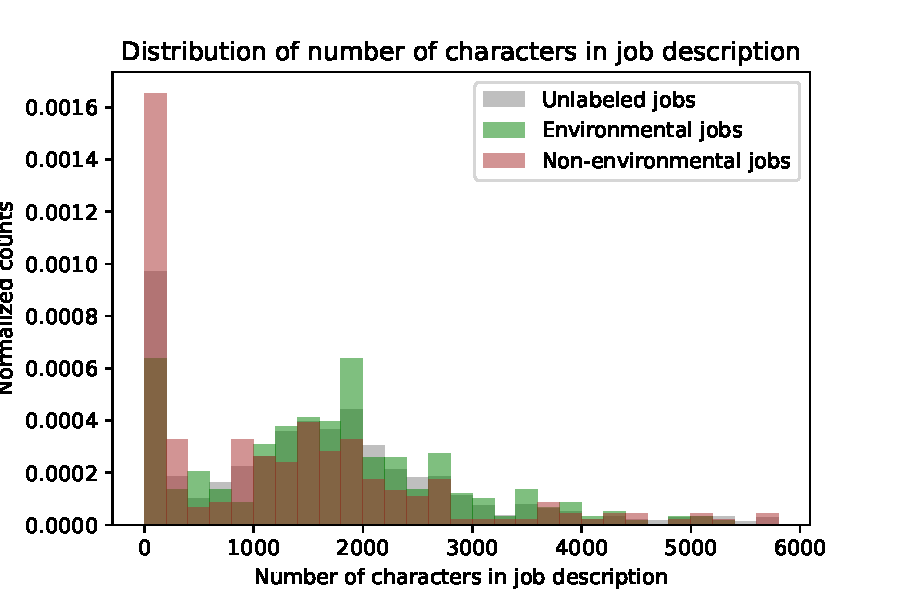
\includegraphics[width=0.49\textwidth]{figures/CharLengthZoomed.pdf}
    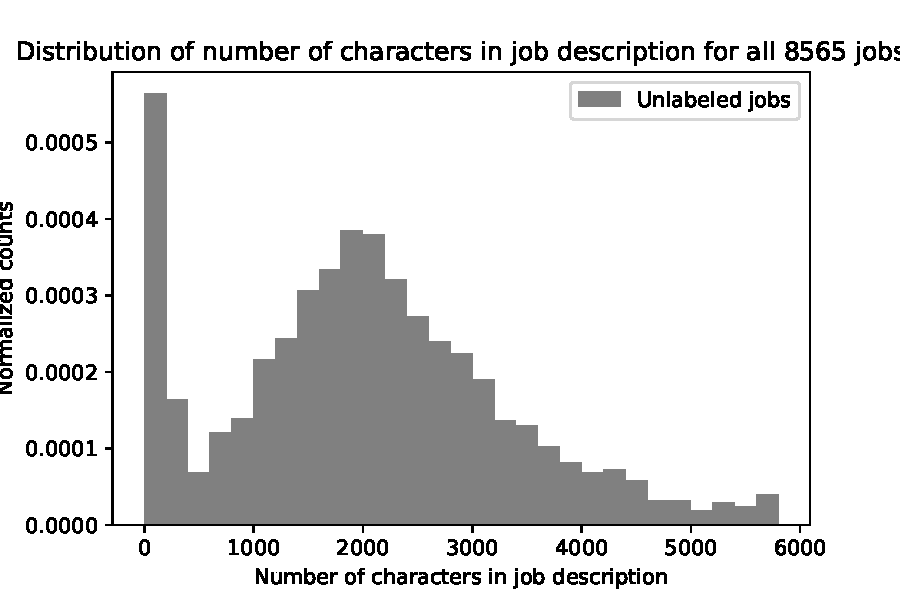
\includegraphics[width=0.49\textwidth]{figures/CharLengthAll.pdf}

    \caption[The distribution of the number of characters in each job description]{
    	The distribution of the number of characters in each job description.
    	The left plot shows the character densities of the 536 labeled jobs. The right plot shows the character densities for all 8568 jobs. 
        Jobs categorized as environmental are shown in green, and those that are not environmental are shown in red. Unlabeled jobs are in grey. 
    }
\label{fig:charlength}
\end{figure}

\label{sec:classification}
\section{Identification of jobs with environmental functions}

Because many of the job offers provided by X28 are not actually environmentally related, a classifier is developed to predict whether or not a given job is relevant to the research question. The aim is to build a classifier that can split the the jobs into environmentally related and non-environmentally related offers. Neural networks are machine learning algorithms named and modeled after the way neurons in the human brain deciphers complex information. These neurons allow the brain to to recognize, categorize, or process certain occurrences in the world around us. Artificial neural networks are designed after this biological function. A simple example of a basic neural network is shown in Fig.~\ref{fig:basicNN}, and is made up of an input layer, one or more hidden layers, and an output layer. 

\begin{figure}[htbp]
  \centering
    \includegraphics[width=0.7\textwidth]{figures/BasicNN.pdf}
    \caption{
    An illustration of a simple neural network with one hidden layer.
    }
\label{fig:basicNN}
\end{figure}



Each neuron, or node of the network, takes numerical input, applies an operation on the input, and outputs a modified value to each neuron to which it is connected. For each connection in the network, the inputs are multiplied by a different numeric value, which constitute the \emph{weights} of the network. The multiplied values are then input to the activation function of the neuron, which provides a non-linear operation for the data, a key aspect that allows the neural network to form a very flexible function capable of predicting complex properties. The activation function effectively determines which neurons are ``activated,'' that is, are above a certain numerical threshold, and therefore pass information to the next layer of neurons as a numerical output. The weights can take different values and are optimized during the training of the model. Several different activation functions can be used, such as the sigmoid or Relu functions. These functions help decide the output of the neurons. 

An simple illustrative example showing how the inputs are transformed in a single node is shown in Fig.~\ref{fig:simplenetwork}. Neural networks can take on a variety of architectures with varying numbers of layers of neurons and different activation functions. The layers can be connected in different ways. In the models utilized for this research, dense, or fully connected layers are used. This means that all the neurons from one layer are connected to all the neurons in the following layer. This is illustrated in Fig.~\ref{fig:fullyconnected}. In classification tasks, the final layer of the network produces numerical values which at different thresholds allow the the model to make different predictions. 

\begin{figure}[htbp]
  \centering
    \includegraphics[width=0.5\textwidth]{figures/SimpleNeuron.pdf}
    \caption{
    An illustrative example of a simple artificial neuron.
    }
\label{fig:simpleneuron}
\end{figure}



\begin{figure}[htbp]
  \centering
    \includegraphics[width=0.3\textwidth]{figures/FullyConnected.pdf}
    \caption{
    An illustrative example of fully connected layers in a neural network.
    }
\label{fig:fullyconnected}
\end{figure}

A neural network model is chosen for the classification of environmentally related and non-environmentally related jobs because of their ability to handle complex, multidimensional data sets, such as human language. They provide the ability to group or classify unlabeled data through unsupervised learning. Human language contains many nuances and complex vocabulary structures, and neural networks have the ability to deal with abstraction.  

Two neural network architectures are developed and compared. The first architecture is the simpler of the two and is shown in Fig.~\ref{fig:simplenetwork}. In this architecture, there is only one input layer, which is the  cleaned and English-translated text of the job offers. The Keras layer encodes the text using the Universal Sentence Encoder~\cite{DBLP:journals/corr/abs-1803-11175}, described further in Section~\ref{sec:activites} using the dedicated Keras interface provided by TensorFlow Hub, and produces an output of a 512-dimensional vector for each sentence. The output of the Keras layer is then fed into the first dense, or fully connected, layer. This means that each input is fed to each individual node, or neuron, of the neural network. These neurons have their own set of weights that are optimized during network training via backpropagation, which when trained helps the neural network learn which features have a more weighted affect on the model's output. The output of the first dense layer therefore are 256 numbers that are obtained by a weighted combination of the vectors and the neurons. All dense layers use the Relu activation function. This simple function, shown in Equation~\ref{eq:relu}, takes a value of 0 for negative inputs, and the input value if the input is positive. 

\begin{equation}
f(x) = \max(0, x)
\label{eq:relu}
\end{equation}

The second dense layer takes in the input of the 256 numbers from the first dense layer, and uses 32 neurons to compute the output, again using a weighted linear combination and the Relu function. Finally, the third dense layer takes in the 32 numbers as an input, and a single node outputs either a 0 or 1 value, using a sigmoid activation function, shown in Equation~\ref{eq:sigmoid}.

\begin{equation}
f(x) = \frac{1}{1+e^{-x}}
\label{eq:sigmoid}
\end{equation}

A value of 0 means that a job offer is classified a non-environmental, and a value of 1 means the job offer is classified as environmental.


\begin{figure}[htbp]
  \centering
    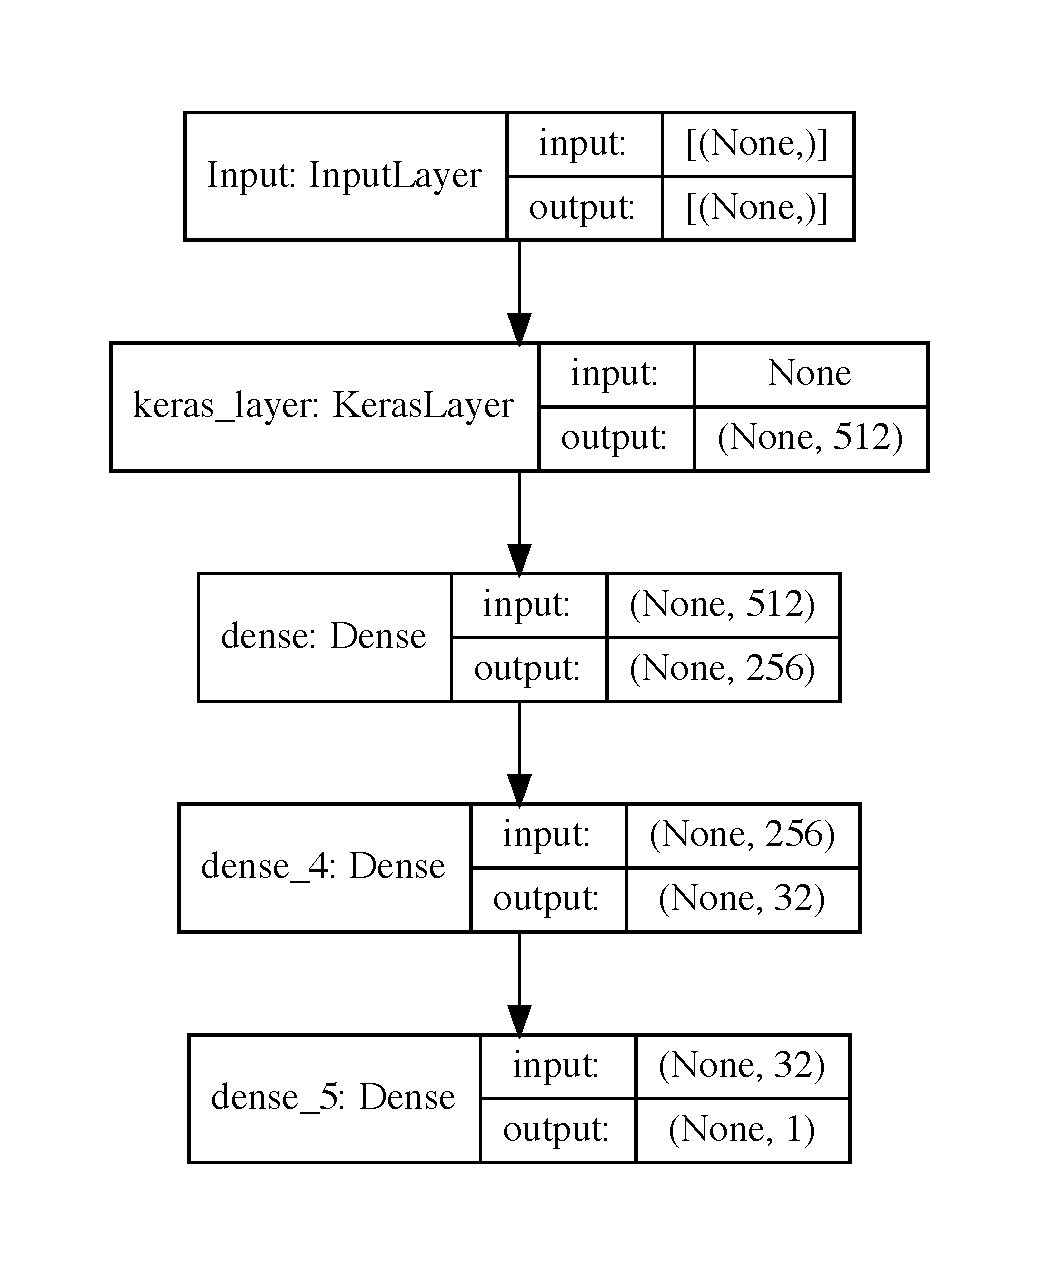
\includegraphics[width=0.7\textwidth]{figures/NeuralNetArch_OnlySentences.pdf}
    \caption[The simpler neural network architecture used in the classification of environmental and non-environmental job offers]{
    The simpler neural network architecture used in the classification of environmental and non-environmental job offers. In this architecture, only the encoded text is used as input.
    }
\label{fig:simplenetwork}
\end{figure}


The second architecture is shown in Fig.~\ref{fig:fullnetwork}. The input layer on the top left refers to the cleaned and translated text of the job offers. The architecture of the network for the layers connected to this input is very similar to the architecture described in Fig~\ref{fig:simplenetwork}. However, this neural network utilizes a separate input layer, labeled input\_1 and shown to the top right of Fig.~\ref{fig:fullnetwork}. This layer takes in a number of other categorical and numeric features of the data. These variables are the number of sentences normalized, the number of characters normalized, the company size represented as a categorical variable, and the canton size represented as a categorical variable. 

\begin{figure}[htbp]
  \centering
    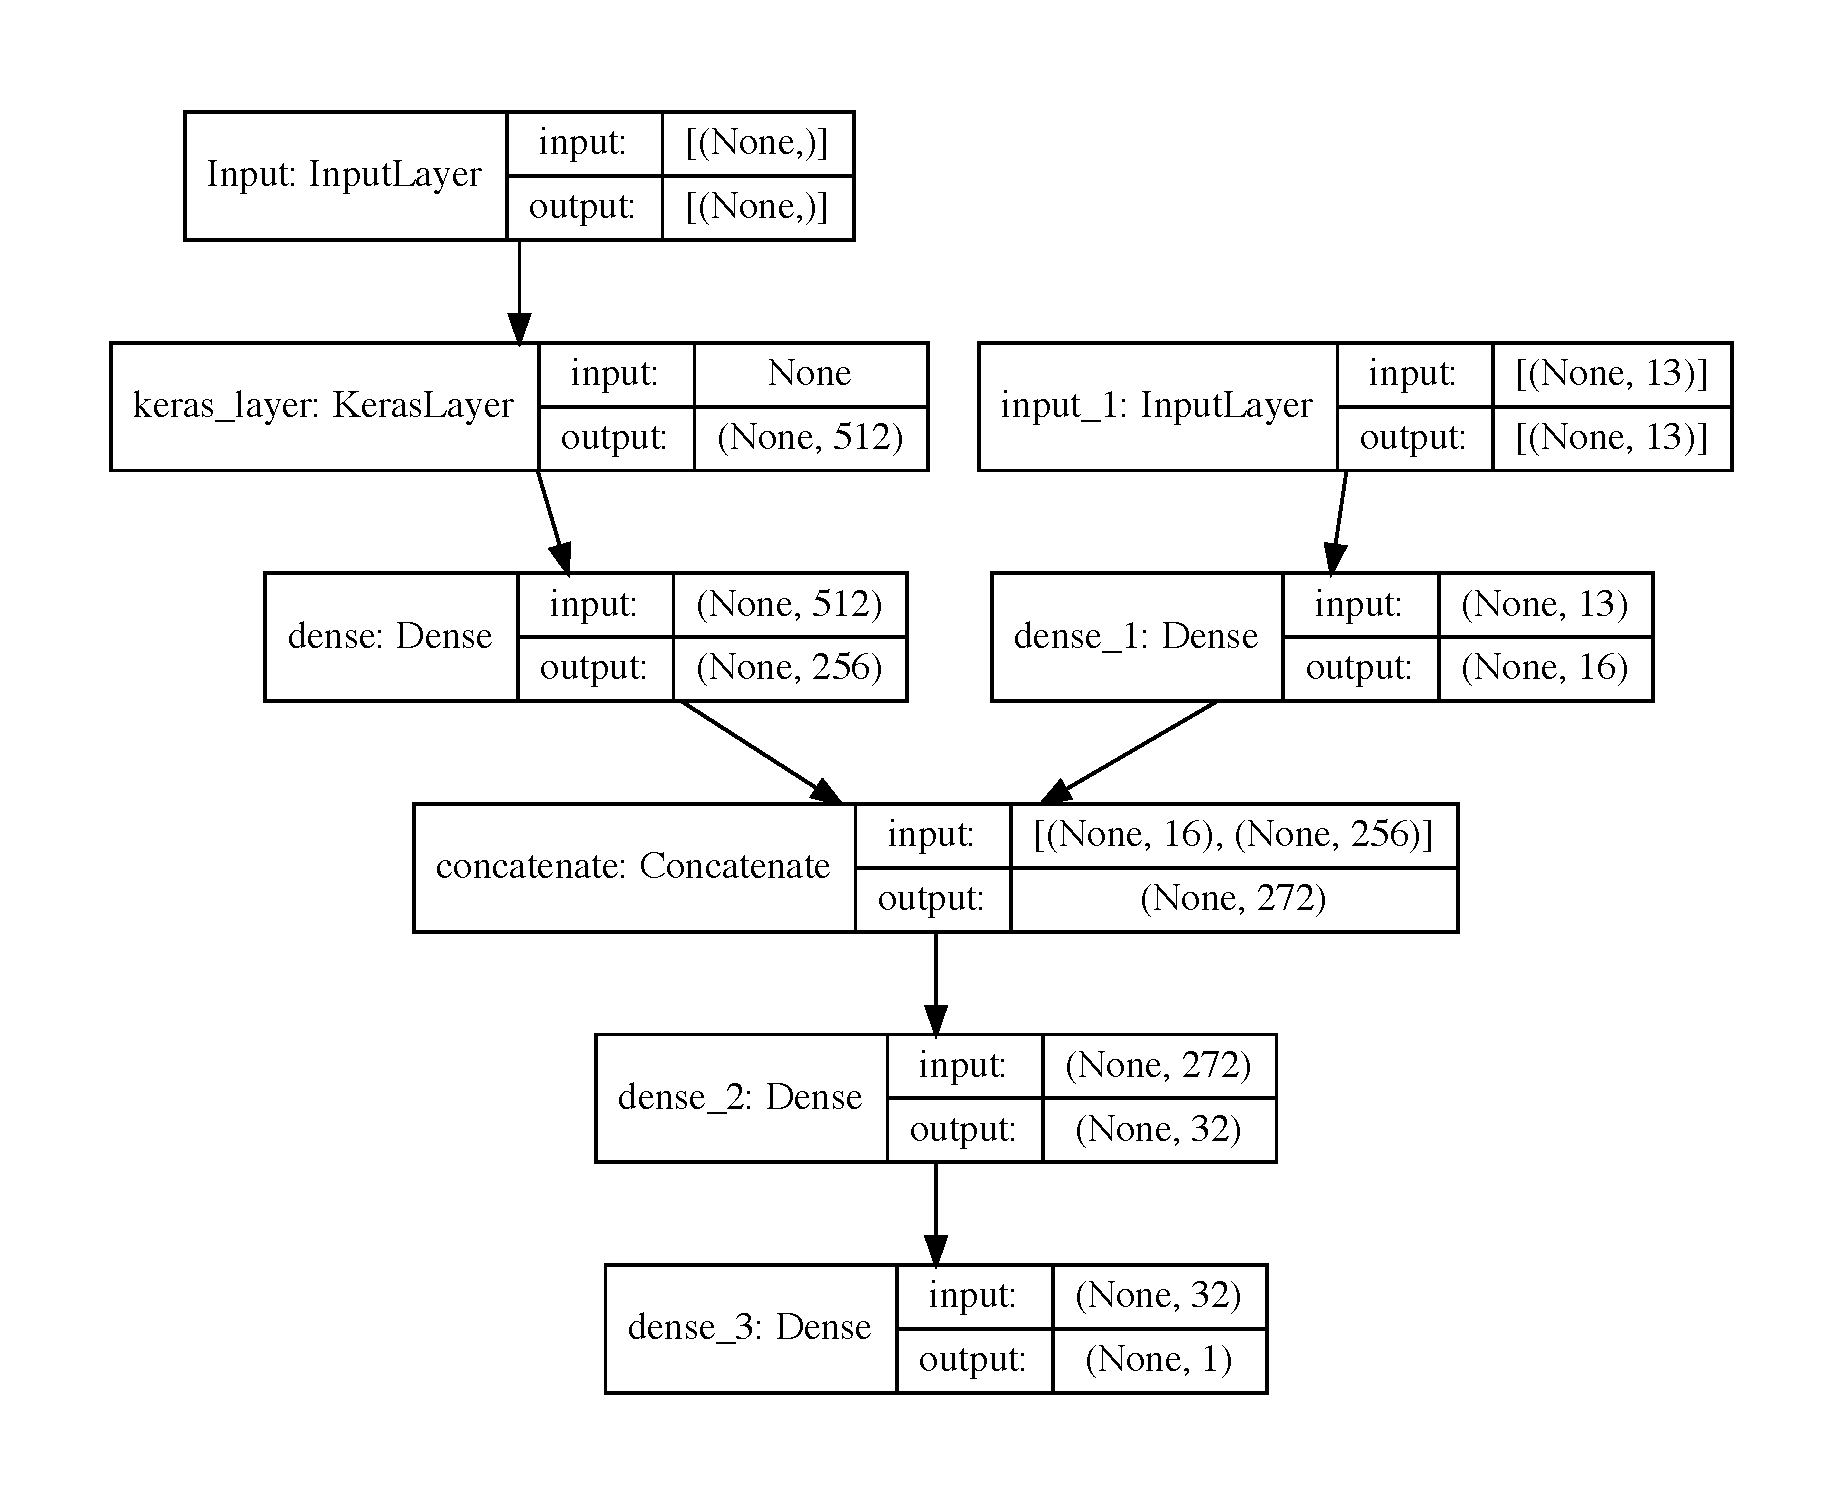
\includegraphics[width=0.7\textwidth]{figures/NeuralNetArch_AllInputs.pdf}
    \caption[The more complex neural network architecture used in the classification of environmental and non-environmental job offers]{
    	The more complex neural network architecture used in the classification of environmental and non-environmental job offers. This architecture takes in the number of sentences in the job offer, the number of characters in the job offer, the size of the company offering the job, and the canton the job is advertised in.
    	}
\label{fig:fullnetwork}
\end{figure}

The number of sentences and the number of characters are normalized by the mean and standard deviation such that the mean and standard deviation are 1. This is done because normalized data is preferred by the neural network, because a large spread in magnitude of input values tends to lead to larger weights in the network and less stable training. The categorical variables are represented by dummy variables rather than by single variables that takes on multiple values. These dummy variables can only take on values of 0 (false) or 1 (true), and as such, they serve the purpose of distinguishing the categories as distinct. Because it is also possible for a company size to be 'uncategorized', the company size variable is represented by four dummy variables. It is not possible for two or more of the dummy variables representing the company size to take a value of 1; however, it is possible for all to be 0, indicating an uncategorized company. For the job's canton, 7 dummy variables indicate whether or not the job takes place in the given canton. It is possible for jobs to cover multiple cantons, or for the job to be in another canton than the 7 most common, which corresponds to a configuration of all dummy variables zero.

Including all the dummy variables, the network considers 13 numeric inputs. The numeric inputs are fed to a dense layer with 16 nodes, which combine the inputs and utilize a Relu activation function, again shown in Equation~\ref{eq:relu}. The 16 numeric outputs of the 16 neurons are concatenated with the 256 numeric results from the dense layer connected to the inputs of the converted sentences to form a concatenated layer of 272 values, as shown inn the center of the figure. These outputs are then fed to a dense layer of 32 neurons before being compressed into a single output layer. The output layer uses a sigmoid activation function, again shown in Equation~\ref{eq:sigmoid}, in  order to compress all inputs to a single number between 0 and 1. The prediction of the network is derived from this result. Values less than 0.5 are then consider false, or not environmentally related in nature, and values greater than 0.5 are taken as environmentally related. 

The use of the Universal Sentence Encoder embeddings allows the model to benefit from the huge training data set used by Google to develop the pre-trained model. However, this data set is not specific to the environment activities categorization task. Through transfer learning, the neural network sculpts the pre-trained inputs towards the task at hand. This approach allows the training to be performant with a much smaller input data set than would be needed to train a NLP model from scratch only using labeled job offers. This approach is essential to this task, because the labeled data set must be tediously constructed by hand, and is therefore of very limited size.

Both models are trained and optimized using the subset of 536 job offers which are labeled as environmentally related or not. Of the 536, 304 are environmentally related, and 237 are not. In order to build a more balanced data set, only two-thirds of the non-environmentally related jobs are used in the training set. A total of 180 job offers are used for the test data set. There are several parameters and hyperparameters that can be optimized within neural network models. These include the learning rate, the number of layers, the batch size, the number of epochs, and the learning rate decay. The learning rate is generally regarded as one of the most important parameters to tune, since it can result in larger performance increases while not adding great amounts of computing time. The number of epochs is also a commonly tuned parameter, with more epochs often improving accuracy, but this usually comes at a higher time cost. Therefore, the learning rate methods and the number of epochs are manipulated in the more complex neural network model in order to improve model accuracy. 

Confusion matrices are made to visualize the performances of the neural network models. A confusion matrix is a table that displays four different combinations of predicted and actual values. The top left quadrant of the confusion matrix displays the number of false predictions which are indeed false. These are called true negative (TN) predictions. The top right quadrant displays the number of true predictions which were actually false. These are called false positive (FP) predictions, or Type I error. The bottom left quadrant displays the number of false predictions which were actually true. These are called false negative (FN) predictions, or Type II error. Finally, the bottom right quadrant displays the number of true predictions which are indeed true. These are called true positive predictions (TP). Using these tallies, it is possible to calculate different metrics to evaluate the models. The recall of the model describes the fraction of relevant instances that are retrieved. The recall equation is shown in Equation~\ref{eq:recall}.

\begin{equation}
\text{Recall} = \frac{TP}{TP + FN}
\label{eq:recall}
\end{equation}

The precision of the model is the fraction of relevant instances among the retrieved instances. The precision equation is shown in Equation~\ref{eq:precision}.

\begin{equation}
\text{Precision} = \frac{TP}{TP + FP}
\label{eq:precision}
\end{equation}

It is ideal to have precision and recall as high as possible, but often they have an inverse relationship. That is why the F-measure is often used as a more holistic metric that combines the precision and recall together. The F-measure equation is shown in Equation~\ref{eq:F}. The F-measure then can be used to identify the best-performing neural network model. 

\begin{equation}
F_{1} = \frac{2 \times \text{Recall} \times \text{Precision}}{\text{Recall} + \text{Precision}}
\label{eq:F}
\end{equation}

The two neural network architectures are compared, with the F-measure taken as the metric of interest to define the optimal model. The hyperparameters of the network, that is, the parameters of the model that are not fixed but are determined by the problem at hand, including the learning rate, number of epochs and batch size, are optimized to achieve the best performance with the labeled data set. The results and the optimal parameters are further discussed in Chapter~\ref{chap:Results}, Section~\ref{sec:greenresults}.

Why don't you add the total number of weights (can get this from model.summary() in Keras)?

You should say what batch size and number of epochs you use. Then you should spend a little bit of effort trying to optimize the network to get the final ac ]] from the two.





\section{Job activity summarizing and skill assessment}
\label{sec:activites}

With ever increasing amounts of textual data available on the Internet, data and computer scientists have focused on developing text mining techniques that require little to no training data. Transfer learning has become a fixture in NLP. This means that the knowledge understood from one model can be applied to a target task downstream, as shown in Fig.~\ref{fig:transferlearning}.

\begin{figure}[htbp]
  \centering
    \includegraphics[width=0.5\textwidth]{figures/transferlearning.pdf}
    \caption{
    An illustration of the concept of transfer learning. 
    }
\label{fig:transferlearning}
\end{figure}


This concept has been one of the main drivers in NLP development as one of the main benefits of using transfer learning is that it reduces the amount of annotated data needed for training a new model. Because human language is so complex, language modeling can be difficult even for humans. The success of many new NLP models is due in part to the fact that they have been built upon existing technology and earlier pre-trained data sets. A good example of this is the performance of Named Entity Recognition models over time, as shown in Fig.~\ref{fig:NERPerformance}.

\begin{figure}[htbp]
  \centering
    \includegraphics[width=1.0\textwidth]{figures/NERPerformance.pdf}
    \caption{
    The performance of Named Entity Recognition models throughout the years. 
    }
\label{fig:NERPerformance}
\end{figure}



One of the most recent models that can handle the task of semantic sentence similarity is Google’s Universal Sentence Encoder (USE). The USE was published in 2018 by a team of Google scientists. The models were pre-trained on a wide range of unsupervised data including Wikipedia pages, question and answer forums, and discussion forums, as well as labeled data allowing supervised learning, including Stanford’s Natural Language Inference corpus. The varied data sources were selected to help make the models more transferable to a wide range of NLP tasks such as semantic sentence similarity, question classification, sentiment analysis and opinion polarity detection of news articles. The model itself encodes English sentences into high dimensional vectors called embeddings. The output of the encoding is 512-dimension vectors, one vector for each encoded sentence. These vectors can then be used to calculate the distance, or similarity, between two sentences based on their cosine distance. This cosine similarity, $\mathrm{sim}(\mathbf{u}, \mathbf{v})$ is a value calculated for two vectors of equal length $\mathbf{u}$ and $\mathbf{v}$ given between -1 and 1 and is calculated with the equation shown in Fig.~\ref{eq:CosineDistance}. The similarity effectively measures the multidimensional angle between two vectors, with values closer to 1 indicating that the vectors are similarly aligned. The cosine distance is defined as  $1 - \mathrm{sim}(\mathbf{u}, \mathbf{v})$. This can be used to determine if  text embeddings have similar properties. The closer the distance is to 1, the more dissimilar the two sentences. Likewise, the more similar the two sentences, the closer the cosine distance is to zero. Values above ones corresponds to sentences that are similar but oppositely aligned. They are uncommon and are not treated in a special way for this analysis, that is, the focus of this analysis is identifying sentences that have cosine similarity distance close to zero. An illustration of the procedure connecting sentence embedding to distance calculation and sentence similarity is shown in Fig.~\ref{fig:USEDiagram}.

\begin{equation}
\mathrm{dist}(\mathbf{u}, \mathbf{v}) = 1 - \mathrm{sim}(\mathbf{u}, \mathbf{v}) = 1 - \frac{1}{\pi}\arccos\left (\frac{\mathbf{u}\cdot \mathbf{v}}{||u|| ||v||}\right)
\label{eq:CosineDistance}
\end{equation}

\begin{figure}[htbp]
  \centering
    \includegraphics[width=1.0\textwidth]{figures/USEDiagram.pdf}
    \caption[A diagram showing how the Universal Sentence Encoder accepts the raw text and embeds the sentences into 512 dimensional vectors]{
    A diagram showing how the Universal Sentence Encoder accepts the raw text and embeds the sentences into 512 dimensional vectors. The vectors allow for the measurement of cosine distance between the sentences. The lower the cosine distance between two sentences, the more semantically similar.
    }
\label{fig:USEDiagram}
\end{figure}


The USE has two methods for performing the encoding. One uses a transformer architecture and the other a Deep Averaging Network (DAN). The transformer based model’s architecture is shown in Fig.~\ref{fig:Transformer}. It was developed by Google in 2017. This architecture is unique because it incorporates a concept called attention. Attention is a mechanism that allows the neural network to focus on a specific subset of features. This means that it gives more 'attention' to some parts or words in the sentence than others, similar to what the human brain does when processing speech and recognizing the most important words. The transformer model was designed to be applied to a number of transfer learning tasks such as text classification and input-response systems. While it is usually more efficient than the DAN architecture, it is often more computationally complex and time consuming.

\begin{figure}[htbp]
  \centering
    \includegraphics[width=0.5\textwidth]{figures/Transformer.pdf}
    \caption{
  The transformer-model architecture.
    }
\label{fig:Transformer}
\end{figure}

The alternative model uses DAN architecture. The word embeddings are averaged and fed through a deep neural network, which produces sentence embeddings.  The sentence embeddings are also vectors of length 512, the same as the attention architecture model. The main advantage to the DAN architecture is that it has a faster processing time, while still having a good performance on a number of transfer tasks. Due to its efficiency, the model that utilizes the DAN architecture was selected for the textual semantic similarity tasks performed in this research. 


As briefly described in the methodology section, a large amount of text cleaning is performed on the job offers data set before using the USE to perform semantic similarity measurements of the job offers to the reference skills and activities data sets compiled from O*Net. Many of the raw job offers contain HTML tags and other extra special characters. An example of the raw text is show in Fig.~\ref{fig:messytext}.

\begin{figure}[htbp]
  \centering
    \includegraphics[width=1.0\textwidth]{figures/MessyText.pdf}
    \caption{
    Raw job offer 12220025, illustrating the presence of HTML tags and special characters in the job offers corpus. 
    }
\label{fig:messytext}
\end{figure}

The first 1000 job offers from the larger corpus are chosen for careful analysis. A function in Python is written to remove the HTML tags and special characters from the text, utlizing the BeautifulSoup HTML parsing package as described in Section~\ref{sec:software}. Another function is written utilizing Google Translate and the Python package EasyMNT to translate the job offers into English. Finally, a third function is written to tokenize the content into individual sentences. An example of this cleaned, translated, and tokenized text is shown in Fig.~\ref{fig:cleanedtext}.

\begin{figure}[htbp]
  \centering
    \includegraphics[width=1.0\textwidth]{figures/cleanedtext.pdf}
    \caption{
    The cleaned, translated, and tokenized job offer 12220025. 
    }
\label{fig:cleanedtext}
\end{figure}

The tokenized job offers are encoded using the USE, as are the sentences corresponding to each individual skill and activity in the O*Net-based data sets. For each job offer, the cosine distance between each sentence, and every single activity and skill is computed. The results are two matrices: one containing the distances between each sentence in the job offers data set and each activity, and the other containing the distances between each sentence in the job offers data set and each skill. In this way, it is possible to identify which sentences in the job offer have the lowest cosine distances to the skills and activities in the reference data sets. For each job offer, the top 10 skills and top 10 activities with the lowest cosine distances to the sentences in the text are ranked. This provides a way to visually inspect idea how many of these skills and activities actually are actually contained in the text of the job offer. Indeed, just because a sentence describing a skill or activity has a low cosine distance to a sentence in the job offer, it does not guarantee that that particular skill or activity is contained in the job offer. An example of a job offer and it's top 10 activity matches are shown in Fig.~\ref{fig:topten}.

\begin{figure}[htbp]
  \centering
    \includegraphics[width=1.0\textwidth]{figures/topten.pdf}
    \caption[Job offer 12220025 and its top 10 activity matches based on lowest cosine distance between the sentence describing the activity, and a sentence in the job offer]{
    Job offer 12220025 and its top 10 activity matches based on lowest cosine distance between the sentence describing the activity, and a sentence in the job offer. The left column shows the cleaned and translated text of the job offer, and the right column shows the activity matches.
    }
\label{fig:topten}
\end{figure}

Because not every skill or activity is contained in each job offer, it is necessary to examine the numerical values of the cosine distances and investigate if there is numerical cutoff that indicates if a skill or activity is relevant to the job. In order to get more stable and reliable skill matches which are not skewed by a single sentence in a particular job offer, top skill matches are calculated by taking the average of the three sentences with the lowest distances. A histogram comparing the cosine distance of the best match skill for each job offer to the cosine distance of all the skills matched to each job offer is shown in Fig.~\ref{fig:SkillHist1}. The histogram clearly demonstrates that the best matched skills tend to have a lower cosine distance than the entire set of all the skills. To define the numerical cutoff between 'relevant' and 'irrelevant' skills for each job offer, the average of the the mean cosine distance and +/- 1 standard deviations is plotted. The cutoff is then defined as the mean cosine minus one standard deviation, or a cosine distance of 0.8158. 


\begin{figure}[htbp]
  \centering
    \includegraphics[width=0.6\textwidth]{figures/SkillHist1.pdf}
    \caption[Comparison of the average distance between the top three sentence matches of all skills and the top three sentence matches to the best skills]{
    The distribution of the average distance between the top three sentence matches of all skills (shown in red), compared to the distribution of the top three sentence matches to the best skills (shown in green). The middle dashed line represents the mean cosine distance for the entire data set. The dashed lines on the left and right refer to the mean minus one standard deviation, and the mean plus one standard deviation, respectively. 
    }
\label{fig:SkillHist1}
\end{figure}

Fig.~\ref{fig:NumSkillsMatches} shows the distribution of the number of matched skills for each job based on the cosine distance cutoff of 0.8158. The majority of the job offers have either 0 matches or more than 10 matches. This large number of jobs without any relevant skills matches could be attributed to the fact that many of the job offers are not of an adequate length and do not describe any details about the job function. 

\begin{figure}[htbp]
  \centering
    \includegraphics[width=0.6\textwidth]{figures/NumSkillsMatches.pdf}
    \caption{
    A histogram showing the distribution of the number of relevant skills matched to the job offers using a cosine distance cutoff of 0.8158. 
    }
\label{fig:NumSkillsMatches}
\end{figure}

Fig.~\ref{fig:SkillGreen} shows the average cosine distance of the sentences in the job offer with the three lowest distances to the environmental skills, by environmental identity. There is a lot of overlap between the distances of the environmental jobs and non-environmental jobs. An reasonable explanation for this could be that many of the skills in reference data set are not mutually exclusive to environmentally related jobs. For example, skill such as, ``managing one's own time and the time of others,'' ``talking to others to convey information effectively,'' ``motivating, developing, and directing people as they work, identifying the best people for the job,'' and ``teaching others how to do something,'' are applicable to jobs in a variety of different sectors. 

\begin{figure}[htbp]
  \centering
    \includegraphics[width=0.6\textwidth]{figures/SkillGreen.pdf}
    \caption{
    The distribution of the average cosine distance of the sentences in the job offer with the three lowest distances to the environmental skills, by environmental identity. 
    }
\label{fig:SkillGreen}
\end{figure}

The same procedure was repeated to find the the relevant activities in the job offers. A histogram comparing the cosine distance of the best match activity for each job offer to the cosine distance of all the activities matched to each job offer is shown in Fig.~\ref{fig:ActivityHist1}. Again, to define the numerical cutoff between 'relevant' and 'irrelevant' activities for each job offer, the average of the the mean cosine distance and +/- 1 standard deviations is plotted. The cutoff is then defined as the mean cosine minus one standard deviation, or a cosine distance of 0.8491.

\begin{figure}[htbp]
  \centering
    \includegraphics[width=0.6\textwidth]{figures/ActivityHist1.pdf}
    \caption[The distribution of the average distance of the top three sentence matches of all activities compared to the top three sentence matches to the best activities]{
     The distribution of the average distance of the top three sentence matches of all activities (shown in red) compared to the distribution of the top three sentence matches to the best activities (shown in green). The middle dashed line represents the mean cosine distance for the entire data set. The dashed lines on the left and right refer to the mean minus one standard deviation, and the mean plus one standard deviation, respectively. 
    }
\label{fig:ActivityHist1}
\end{figure}

Fig.~\ref{fig:NumSkillsMatches} shows the distribution of the number of matched activities for each job based on the cosine distance cutoff of 0.8491. The majority of the job offers have either 0 matches or more than 10 matches, similarly to the number of skills matches.

\begin{figure}[htbp]
  \centering
    \includegraphics[width=0.6\textwidth]{figures/NumActivitiesMatches.pdf}
    \caption{
    The distribution of the number of relevant activities matched to the job offers using a cosine distance cutoff of 0.8491. 
    }
\label{fig:NumActivityMatches}
\end{figure}

Furthermore, Fig.~\ref{fig:ActivityGreen} shows the average cosine distance of the sentences in the job offer with the three lowest distances, by environmental identity. Though there is some overlap, in general the environmentally related jobs have a lower cosine distances to the activities in the reference data set, meaning the environmentally related jobs are more semantically similar. This is an encouraging result and suggests the neural net classifier indeed is able to identify job offers that contain environmental activities as environmental in nature. 

\begin{figure}[htbp]
  \centering
    \includegraphics[width=0.6\textwidth]{figures/ActivityGreen.pdf}
    \caption{
    The average cosine distance of the sentences in the job offer with the three lowest distances to the environmental activities, by environmental identity. 
    }
\label{fig:ActivityGreen}
\end{figure}







%%%%%%%%%%%%%%%%%%%%%%%%%%%%%%%%%%%%
\chapter{Results}

This section gives the results of the primary tasks of this thesis: the classification of jobs according to whether or not they include environmental activities, described in Section~\ref{chap:procedure}, and the association of jobs to activities and skills, the procedure of which is outlined in Section~\ref{sec:activites}.

The full results for all 8565 jobs in the data set can be found in the Results folder of the repository in Ref~\cite{emilysharata}. Only a small labeled data set is available for the categorization task. For the association of jobs to skills, the performance is assessed by manually inspecting a small, random subset of the results. Additional labeling and inspection of the results is possible on the full data set, which is made available, but is outside the scope of the present discussion.
\label{chap:Results}
%%%%%%%%%%%%%%%%%%%%%%%%%%%%%%%%%%%%
\section{Environmental job classification}
\label{sec:greenresults}

To have an understanding of a baseline neural network performance for this particular classification task, inspection of the confusion matrix of the simpler neural network model described in  is used. This model uses the Adam adaptive learning rate method and three epochs. The confusion matrix is shown in Fig~\ref{fig:simpleModelConfusion}. The F-measure for this model is 0.785.


\begin{figure}[htbp]
  \centering
    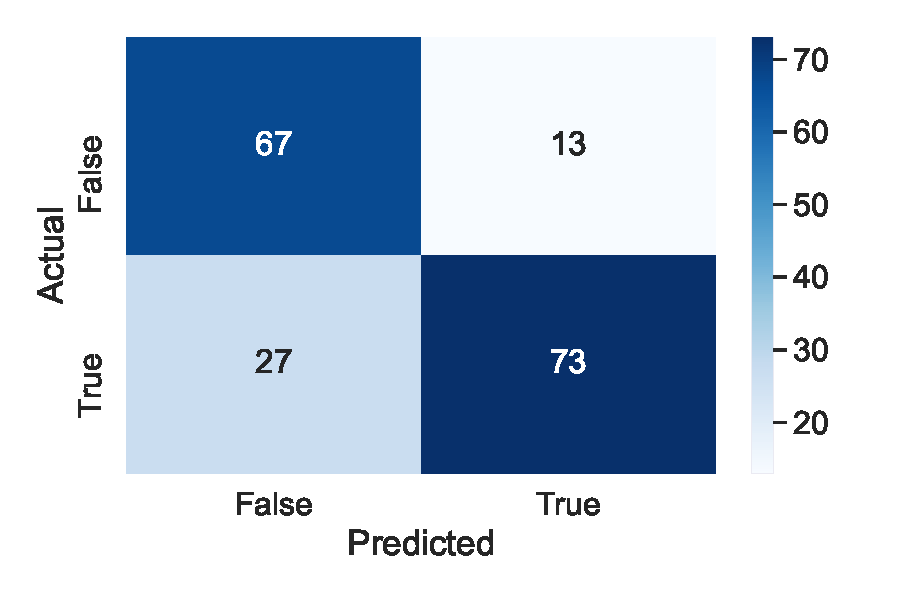
\includegraphics[width=0.5\textwidth]{figures/simpleModelConfusion.pdf}
    \caption{
    	The confusion matrix of the simpler neural network model, using 3 epochs and the Adam optimizer. 
    	}
\label{fig:simpleModelConfusion}
\end{figure}

The more complex neural network model is then optimized by changing the adaptive learning rate method and the number of epochs. Four different combinations are evaluated: The Adam optimizer with three epochs (Fig~\ref{fig:Complex3Adam}), the Adam optimizer with six epochs (Fig~\ref{fig:Complex6Adam}), the RMS Prop optimizer with three epochs (Fig~\ref{fig:Complex3RMSProp}), and the RMS Prop optimizer with six epochs (Fig~\ref{fig:Complex6RMSProp}). The 

The Adam and RMS Prop optimizers produce similar results, although the number of true negatives 

\begin{figure}[htbp]
  \centering
    \includegraphics[width=0.5\textwidth]{figures/Complex3Adam.pdf}
    \caption{
    	The confusion matrix of the more complex neural network model, using 3 epochs and the Adam optimizer. The F-measure for this model is 0.799.
    	}
\label{fig:Complex3Adam}
\end{figure}

\begin{figure}[htbp]
  \centering
    \includegraphics[width=0.5\textwidth]{figures/Complex6Adam.pdf}
    \caption{
    	The confusion matrix of the more complex neural network model, using 6 epochs and the Adam optimizer. The F-measure for this model is 0.800.
    	}
\label{fig:Complex6Adam}
\end{figure}

\begin{figure}[htbp]
  \centering
    \includegraphics[width=0.5\textwidth]{figures/Complex3RMSProp.pdf}
    \caption{
    	The confusion matrix of the more complex neural network model, using 3 epochs and the RMS Prop optimizer. The F-measure is 0.803.
    	}
\label{fig:Complex3RMSProp}
\end{figure}

\begin{figure}[htbp]
  \centering
    \includegraphics[width=0.5\textwidth]{figures/Complex6RMSProp.pdf}
    \caption{
    	The confusion matrix of the more complex neural network model, using 6 epochs and the RMS Prop optimizer. The F-measure is 0.801.
    	}
\label{fig:Complex6RMSProp}
\end{figure}


Although all very similar in performance, the model with the highest F-measure is the more complex model using three epochs and the RMS Prop optimizer. With an F-measure of 0.801, it slightly outperforms the other models.


\section{Job skill and activity association}
\label{sec:activityresults}

In order to identify the relevant skills and activities in the job offers text, the cosine distance cutoffs found and discussed in Section~\ref{sec:activites} are used. Using the cosine distance cutoff of 0.8491, the number of activity matches can be compared to the top 10 activity matches by distance. Fig.~\ref{fig:AllActMatches13763695} shows the top 10 activity matches to the job offer 13763695. Fig.~\ref{fig:GoodActMatches13763695} shows the activity matches to the job offer 13763695 using the cosine distance cutoff. Certain activities in the the diagram showing the top 10 best matched activities are clearly irrelevant to the job offer. For example, ``apply protective coatings,'' is not contained in the text although it is the 10th most semantically similar sentence to the sentences in the job offer. 

\begin{figure}[htbp]
  \centering
    \includegraphics[width=1.0\textwidth]{figures/AllActMatches13763695.pdf}
    \caption[The top 10 activity matches to the job offer 13763695]{
    The top 10 activity matches to the job offer 13763695. The content of the job offer is shown on the left, and the activity matches are shown on the right. 
    }
\label{fig:AllActMatches13763695}
\end{figure}

\begin{figure}[htbp]
  \centering
    \includegraphics[width=1.0\textwidth]{figures/GoodActMatches13763695.pdf}
    \caption[The activity matches to the job offer 13763695 using the cosine distance cutoff of 0.8491]{
    The activity matches to the job offer 13763695 using the cosine distance cutoff of 0.8491. The activity matches are shown on the left, and the content of the job offer is shown on the right. 
    }
\label{fig:GoodActMatches13763695}
\end{figure}

For the skills, the same comparison is made between the top ten matches by distance and the skills matches with the cosine cutoff distance of 0.8158. Fig.~\ref{fig:GoodSkillMatches} shows the top ten skills matches for job offer 13763695. In this particular case, the top ten best matched skills are all within the 0.8158 cutoff, as the matches are exactly the same. The is not an unusual result, as there can be many skills that can be legitimately applicable to each job offer. 

\begin{figure}[htbp]
  \centering
    \includegraphics[width=1.0\textwidth]{figures/GoodSkillMatches.pdf}
    \caption[The skill matches to the job offer 13763695 using the cosine distance cutoff of 0.8158]{
    The skill matches to the job offer 13763695 using the cosine distance cutoff of 0.8158. The activity matches are shown on the right, and the content of the job offer is show on the left. 
    }
\label{fig:GoodSkillMatches}
\end{figure}

With a visual inspection, it is clear that many of these matched skills and activities are indeed relevant, especially the top one or two matches (i.e., those with the lowest cosine similarity scores, shown at the beginning of the listed skills). However, there still exists some room for matching refinement. For example, the activity match ``performing day-to-day administrative tasks such as maintaining information files and processing paperwork'' is best matched with the sentence from the sentences in the job offer `do not hesitate to send your full application file with motivation file' and 'curriculum vitae copies of diplomas and work certificates via Jobup only.' In this case, these sentences inn the job offer are only referring to the application procedure, and not the functions of the job itself. Therefore, in future research it will be necessary to either further experiment with the cutoff cosine distances, or perhaps more practically, develop a method to remove the irrelevant parts of the job offers text. The full results of the relative skills and activities identification can be found 

\chapter{Conclusions and future prospects}
\label{sec:conclusions}
This thesis has presented a method for classifying job offers advertised in Switzerland and a method for identifying the relevant skills and activities in the job offers. A general software framework has been developed for this task, found in Ref.~\cite{emilysharata}. This framework was designed to enable each step in the analysis tasks of this research project. In particular, the job offers were cleaned of non-alphanumeric characters and converted to numeric data useful for automated natural language processing tasks before applying machine-learning techniques and interpreting the results.

Two neural network models were built for the classification task. The more complex model was tuned by changing the learning rate optimizer method and the number of epochs. The neural network using the RMS Prop optimizer and three epochs performed the best with an F-measure of 0.803. Google's Universal Sentence Encoder was used for the skills and activities identification. By measuring the cosine distance between the encoded sentences of the job offer texts and the sentences of the skills and activities references, the skills and activities with the highest semantic similarity to job offer, and thus the most relevant, were identified. By inspecting the results for a small, random subset of the jobs and tasks, it has been demonstrated that this technique is viable for the categorization and association of jobs to skills and activities.

There were several challenges posed by this research question. The job offers data set had many complications. This data set compiled by X28 was intended to only contain environmentally related job offers, but also contained job offers from unrelated sectors as well as incomplete or unintelligible job descriptions. This created a need to develop a classifier to identify whether a job offer was environmentally related or not. For the classification task, there were only 536 labeled job offers. Labeling the data was labor and time intensive and therefore the number of labeled data was extremely limited. This made the test and train data sets relatively small, making it difficult to adequately train and deploy the model.

For the semantic textual similarity measures between the job offers text and the activities and skills texts, the main challenge was the lack training data. Without this, it was not possible to quantitatively score the performance of the USE model's ability to identify the relative skills and activities in the text. Given the large number of reference skills and activities, as well as the length of the text of some of the job offers, the labeling of the data for semantic similarity would be extremely challenging and time consuming. Therefore, only a qualitative manual inspection of the results was possible. 

Despite the limitations of the data set, this research has demonstrated incredible abilities of transfer learning with pre-trained models. By manually inspecting a small subset of the associated activities and skills, it is clear that the USE does encode relevant information, and that this technique is a viable one to simplify and automate the association of environmental jobs to tasks and skills. In addition, this work has established a usable software setup to continue to explore the data set, and a baseline procedure to accomplish this task.

Moving forward, this work could be expanded in several ways. A larger labeled data set would facilitate the development of a more robust neural net classification model, and would allow for the possibility to score the USE models quantitatively with the F-measure. As is the challenge with many NLP tasks, it is difficult to quantitatively evaluate their performances. Another way future research could be expanded is through a more thorough cleaning of the job offers. Despite removing special characters and translating the text, many job offers still contained irrelevant numbers, URLs, or other unintelligible text. Furthermore, it could be worthwhile to develop a method to remove the part of the job offer that describes the company, so that the focus of the semantic similarity measure is only between the part of the text that describes the job function and the skills and activities. This could in principal also improve the accuracy of the neural network classifier. 
With additional time, it would be worthwhile to explore additional neural network architectures or even different types of classifiers. Support vector machines, decision trees, or logistic regression could be investigated for the classification task. With regards to the textual semantic similarity between the job offers and the skills and activities, different pre-trained NLP encoders could be deployed, evaluated and compared. Finally, more research could be done to improve the cosine distance cutoff values to distinguish between the relevant and irrelevant skills and activities within the job offers text. With additional time, it is possible that choosing different cut off values based on the length of the job offer text, the type of sector the job is in, or the canton of the job offer could offer better results. All in all, this research has shown great promise and has demonstrated the abilities of machine learning and NLP to help researchers gain a better understanding of the current state of environmentally focused job opportunities within Switzerland.  

\vfill

\printbibliography[title=References]\addcontentsline{toc}{chapter}{References}


\end{document}
